\setcounter{ExampleCounter}{1}
\marginnote{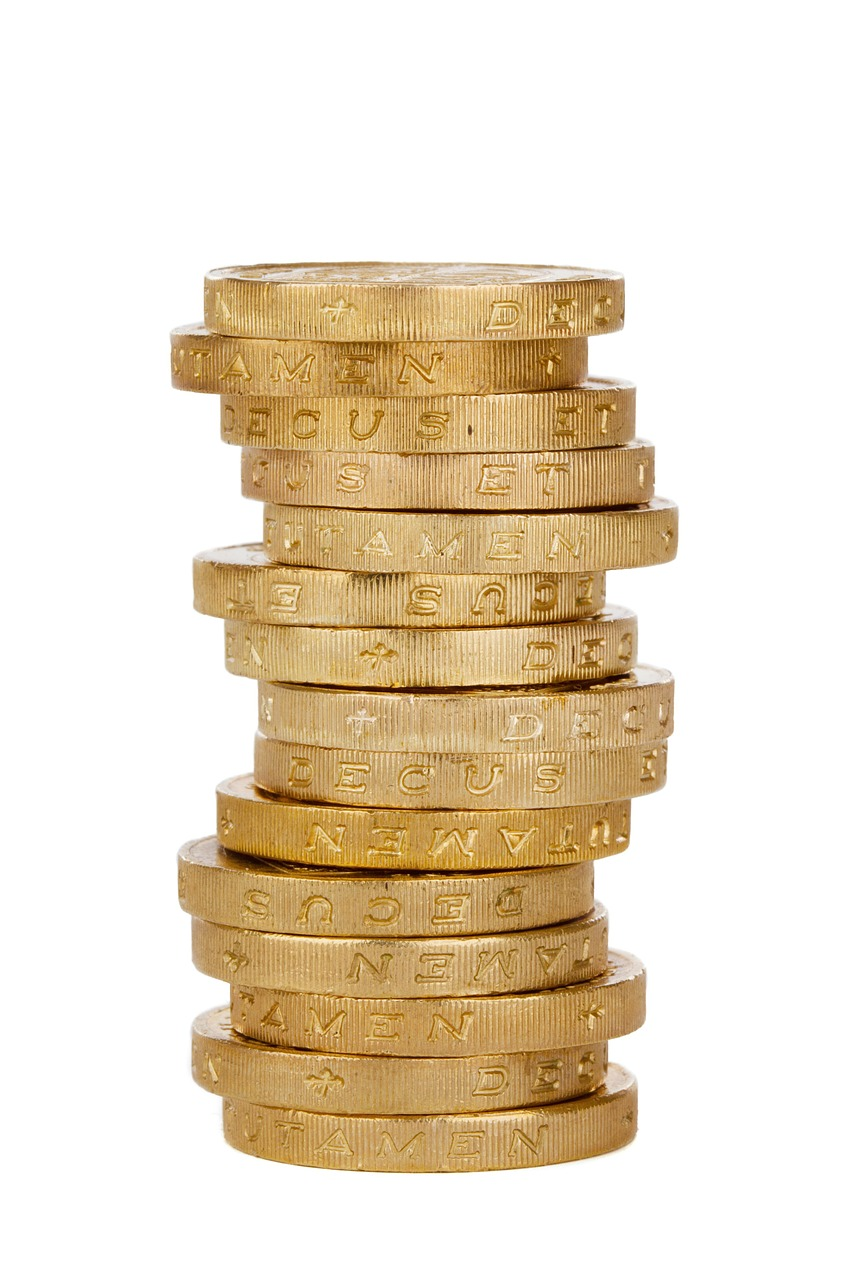
\includegraphics[scale=0.05]{Coins1}}
The basic goal of business (as simplistic as it sounds) is to take a small pile of money and turn it into a big pile of money.  This is capitalism explained in a single sentence.  Because of that, there is value to holding money, because you can use it to make more money.\\  

For instance, say you want to start a landscaping business.  It's unlikely that you would have enough money lying around to do so, so you would take out a small business loan and use that money to buy a truck, a trailer, lawn mowers, blowers, rakes, etc.  Maybe you'd even hire a few employees with that starting capital.  However, you wouldn't sit on that pile of cash; instead, you'd use it to acquire that equipment that you'd use to generate revenue by mowing lawns, raking leaves, removing stumps, and so on.  \marginnote{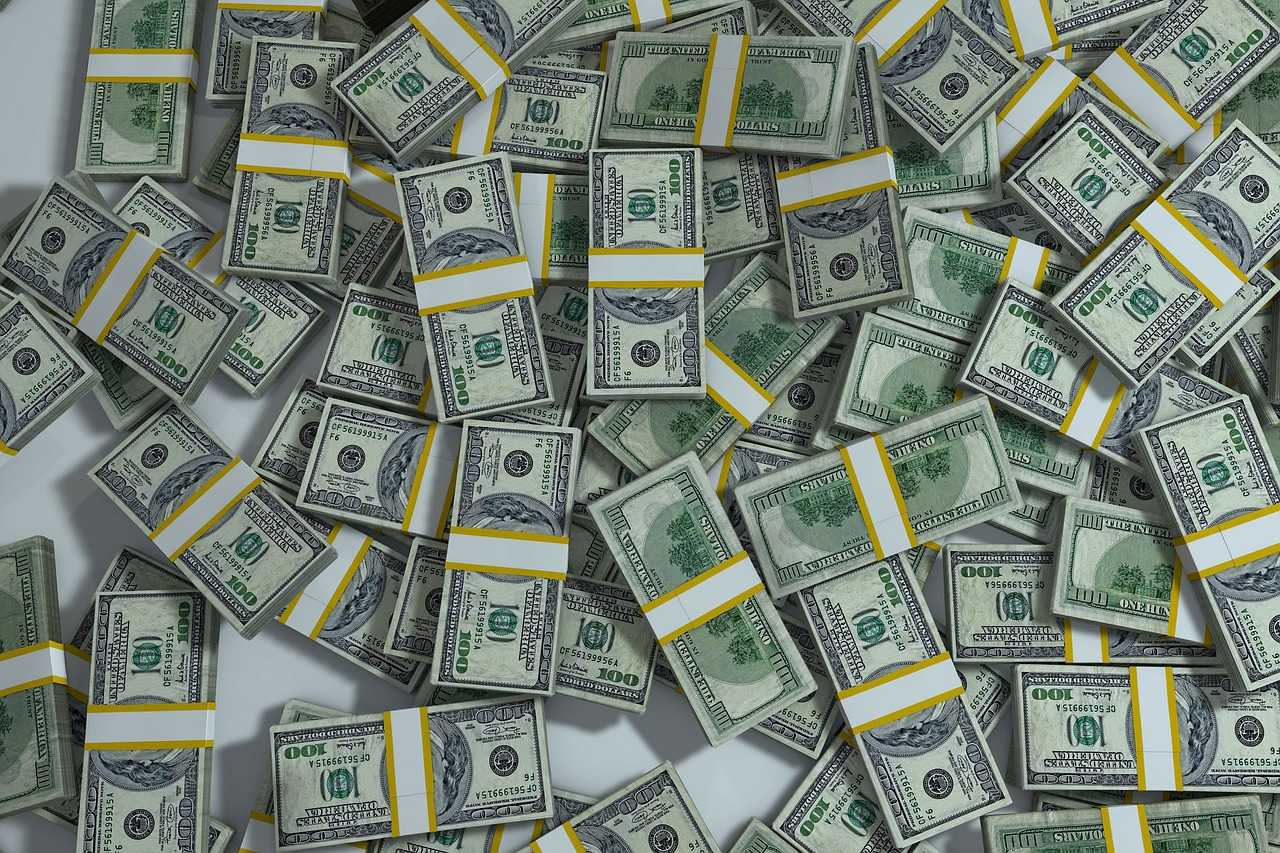
\includegraphics[scale=0.07]{MoneyPile1}}Your goal would be to make more money than you took out as a loan; that way, when you pay back the loan, you'll have a little left over to pay your employees and yourself.

\paragraph{Time Value} We say then that money has \textit{time value}, meaning that if I have a certain pile of money, I expect it to grow over time if I use it properly.  Since everyone treats money this way, if I want to borrow someone else's money and use it for some time, I need to pay them back for the money that they could have made off of it.  This is where \textit{interest} comes into play.  Interest is essentially the price we pay to use someone else's money---think of it as renting their money.  This works both ways---if I want to buy a house, I need money right now, so I borrow from a bank, but I have to, over time, pay them not only the money I borrowed, but also the money they expected to make off of it through their own investments.  Likewise, when I place my money in a bank account, the bank pays me interest in return for being able to use that money to invest and make their pile of money a bit bigger.  Thus, we talk about the \textit{present value} of money, and its \textit{future value}.  The future value is hopefully greater than the present value, since money gains value over time (assuming that inflation doesn't wipe out that gain).

Since interest is given as a rate, the amount of interest you would owe on a particular loan depends on the size of the loan (the interest is a percentage of the amount you take out).

\begin{proc}{Vocabulary}
\begin{itemize}
\item \textbf{Principal:} The amount of money that is borrowed.  This can be paid back in one lump sum, or gradually over time.
\item \textbf{Simple Interest:} Interest that is calculated based on the principal alone.
\item \textbf{Compound Interest:} Interest that is calculated based on the principal and the accumulated interest.
\end{itemize}
\end{proc}

\subsection{Simple Interest}
Suppose you take out a loan for \$500 at 10\% annual interest rate for 4 years.  Each year, (\$500)(0.1) = \$50 in interest accrues, so the total interest is 4 times this:
\[(\$500)(0.1)(4) = \$200\]
At the end of the 4 years, you'll have to pay back the principal, \$500, plus the interest, \$200, for a total of \$700, so a present value of \$500 grew to a future value of \$700.  Clearly, this growth depends on the interest rate and the amount of time involved.

\begin{formula}{Simple Interest}
The interest, $I$, earned on a loan with principal $P$ at annual interest rate $r$ (expressed as a decimal) over a period of $t$ years is
\[I=Prt\]
This formula works with other time periods (months, for instance) as long as the interest rate is given in the same terms (so a monthly interest rate, for instance).

\paragraph{Future Value}
The future value ($F$) of this principal (or present value) $P$ is the sum of the principal and the interest:
\begin{align*}
F &= P + Prt\\
F \marginnote{Future value for simple interest}&= P(1+rt)
\end{align*}
Other kinds of loans (like compound interest) will have different formulas for future value, but the principal is the same: this formula tells how this money will grow.
\end{formula}

\paragraph{APR: Annual Percentage Rate} Note carefully that $t$ is measured in \textit{years}; this is consistent for almost all the financial formulas in this chapter.  This means that interest rates are given as \textit{annual} interest rates.  It's also possible to express loans in monthly terms.  To do so, the APR is divided into a monthly interest rate; for example, a 12\% APR would be 1\% monthly, a 6\% APR would be 0.5\% monthly, etc.

\begin{example}[https://www.youtube.com/watch?v=TJqhAMb2T6Q]{Simple Interest}
\marginnote{\includegraphics[scale=0.15]{TNote1}}
Treasury notes and savings bonds are issued by the federal government to cover its expenses and debt.
Suppose you obtain a \$1,000 Series EE savings bond with a 4\% annual rate and sell it 8 years later. How much interest will you earn?\\
\vspace{0.2in}

\marginnote{\bfseries Solution}
Use the simple interest formula above:
\begin{align*}
I &= Prt\\
&= (\$1000)(0.04)(8)\\
&= \$320
\end{align*}

You'll earn \$320 in interest, so at the end you'll have a total of \$1320.
\end{example}

\begin{try}[http://izzomath.com/103text/finance/example3.1/story.html]
You deposit \$3000 in a savings account at BB\&T Bank, earning 5\% interest.  Find the amount of interest earned and the total amount in the account after three years.
\end{try}

\begin{example}[https://www.youtube.com/watch?v=T4BcmTGwJCI]{Future Value with Simple Interest}
If you deposit \$6200 at 6\%, what is the future value of the deposit at the end of 2.5 years?\\

\marginnote{\bfseries Solution}
Rather than calculating the interest first and adding that onto the principal, we can use the future value formula to do both steps at once:
\begin{align*}
F &= P(1+rt)\\
&= \$6200(1+(0.06)(2.5))\\
&= \$7130
\end{align*}
\end{example}

\begin{try}[http://izzomath.com/103text/finance/example3.2/story.html]
What is the future value of \$2400 at 7\% simple interest at the end of three years?
\end{try}

\begin{example}[https://www.youtube.com/watch?v=0GFzH0JPYeY]{Present Value with Simple Interest}
You'd like to buy a \$12,000 car in 18 months, and your bank is offering 6\% simple interest.  How much should you deposit now in order to have a final balance of \$12,000?\\

\marginnote{\bfseries Solution}
\marginnote{\includegraphics[scale=0.15]{VWVan1}}
We can use the same future value formula as in the previous example, but now the future value is given, and the present value is the unknown part:
\begin{align*}
F &= P(1+rt)\\
\$12,000 &= P(1+(0.06)(1.5))\\
\end{align*}
Now solve this for $P$ to find the amount that you need to deposit today:
\begin{align*}
\$12,000 &= P(1.09)\\
\dfrac{\$12,000}{1.09} &= P = \$11,009.17
\end{align*}
You'll need to deposit \$11,009.17 today in order to have \$12,000 in the account in 18 months.
\end{example}

\begin{try}[http://izzomath.com/103text/finance/example3.3/story.html]
How much do you need to deposit today in an account earning 3\% simple interest to have \$800 in 36 months?
\end{try}

\subsection{Compound Interest}
With simple interest, we assumed that we pocketed the interest when we received it.  If, on the other hand, we added that interest to the account, we could earn interest on that interest in the future, making the balance grow a little bit faster.  This reinvestment of interest is called \textbf{compounding}.\\

Suppose we deposit \$5000 for 5 years in an account offering an 8\% APR, with interest compounded yearly.  How much will be in the account at the end?

At the end of each year, 8\% of the balance at that point will be added to the account, and the balance will grow.  The following table shows on a year-to-year basis the total dollar amount in the account at the end of each year and the interest that accrues that year.
\begin{center}
\begin{tabular}{| c | p{1in} | p{1.52in} | p{1.5in} |}
\hline
{\small Year} & {\small Starting Balance} & {\small Interest Earned} & {\small Final Balance}\\
\hline
1 & \$5000 & $\$5000 \times 0.08 = \$400$ & $\$5000 + \$400 = \$5400$\\
\hline
2 & \$5400 & $\$5400 \times 0.08 = \$432$ & $\$5400 + \$432 = \$5832$\\
\hline
3 & \$5832 & $\$5832 \times 0.08 = \$467$ & $\$5832 + \$467 = \$6299$\\
\hline
4 & \$6299 & $\$6299 \times 0.08 = \$504$ & $\$6299 + \$504 = \$6803$\\
\hline
5 & \$6803 & $\$6803 \times 0.08 = \$544$ & $\$6803 + \$544 = \$7347$\\
\hline
\end{tabular}
\end{center}
The total amount in the account at the end of the fifth year is \$7347, which is \$347 more than we would have earned using simple interest.  Notice that each year, the amount of interest that we earned grew, making the account grow faster and faster.  This is the advantage of compounding, and over long periods of time it can lead to very dramatic results.\\

Following this example, we can derive a formula to take care of the calculation for us so that we don't have to build a table like this every time.  At the end of the first year, the balance had grown to \[\$5000+(\$5000)(0.08) = \$5000(1+0.08).\]  Following the pattern, each year the balance is multiplied by $(1+0.08)$, so at the end of the second year, the balance grew to 
\[\$5000(1+0.08)(1+0.08) = \$5000(1+0.08)^2.\]  At the end of the third year, then, the account would hold $\$5000(1+0.08)^3$, and so on.

After $t$ years, the amount in an account with an interest rate of $r$, compounded once per year, will be\marginnote{Future value for interest compounded yearly} \[F=P(1+r)^t\]

\paragraph{What if interest isn't compounded yearly?} The formula we just derived assumes that interest is compounded---or added to the account---at the end of each year.  However, this doesn't have to be the case; interest could be compounded twice a year (semiannually), four times a year (quarterly), monthly, weekly, or even daily.  \marginnote{\begin{tabular}{r | l}
{\small Compounded} & $n$\\
\hline
{\small Annually} & 1\\
{\small Semiannually} & 2\\
{\small Quarterly} & 4\\
{\small Monthly} & 12\\
{\small Weekly} & 52\\
{\small Daily} & 365\footnotemark
\end{tabular}}\footnotetext{Before calculators were commonplace, some calculations used $n=360$ for daily compounding to make the arithmetic simpler} keep track of how often interest is compounded, we define $n$ as the \textbf{number of times per year that interest is compounded}, regardless of how many years the account grows.

Now if we split the year into $n$ segments, the interest rate will be divided up as well, so each segment will earn an interest rate of $\frac{r}{n}$, so that will replace $r$ in the compound interest formula.  Also, rather than having the interest accrue $t$ times, it will accrue $n$ times each year for $t$ years, or a total of $nt$ times, so that will replace $t$ in the compound interest formula.
\vspace{0.5in}

All of this brings us to the complete formula for the future value of an investment with compound interest.
\begin{formula}{Compound Interest}
The future value $F$ of a principal amount $P$ with an annual interest rate $r$ (expressed as a decimal) compounded $n$ times per year for $t$ years is
\[F=P\left(1+\dfrac{r}{n}\right)^{nt}\]
Notice that if interest is compounded yearly, $n=1$, and the formula becomes the one we derived after the example above.
\end{formula}
\vfill

\begin{example}[https://www.youtube.com/watch?v=UCQJgC0nRxA]{Certificate of Deposit}
A certificate of deposit (CD) is an account that many banks offer that often comes with a higher interest rate, but the investment cannot be touched for a specified length of time.  Suppose you deposit \$3000 in a CD earning 6\% interest compounded monthly.  How much will you be able to withdraw at the end of 20 years?\\

\marginnote{\bfseries Solution}
List the pieces of the formula that are given:
\begin{center}
\begin{tabular}{l l}
$P$ & \$3000\\
$r$ & 0.06\\
$n$ & 12\\
$t$ & 20
\end{tabular}
\end{center}
So at the end of the 20 years, the account will hold 
\[F = 3000\left(1+\dfrac{0.06}{12}\right)^{(12)(20)} = \$9930.61\]

Now compare this to the amount you would earn from simple interest.
\begin{center}
\begin{tabular}{l | r | r}
Years & Simple Interest & Compound Interest\\
\hline
5 & \$3900 & \$4046.55\\
10 & \$4800 & \$5458.19\\
15 & \$5700 & \$7362.28\\
20 & \$6600 & \$9930.61\\
25 & \$7500 & \$13,394.91\\
30 & \$8400 & \$18,067.73\\
35 & \$9300 & \$24,370.65
\end{tabular}
\end{center}
\pagebreak

\begin{center}
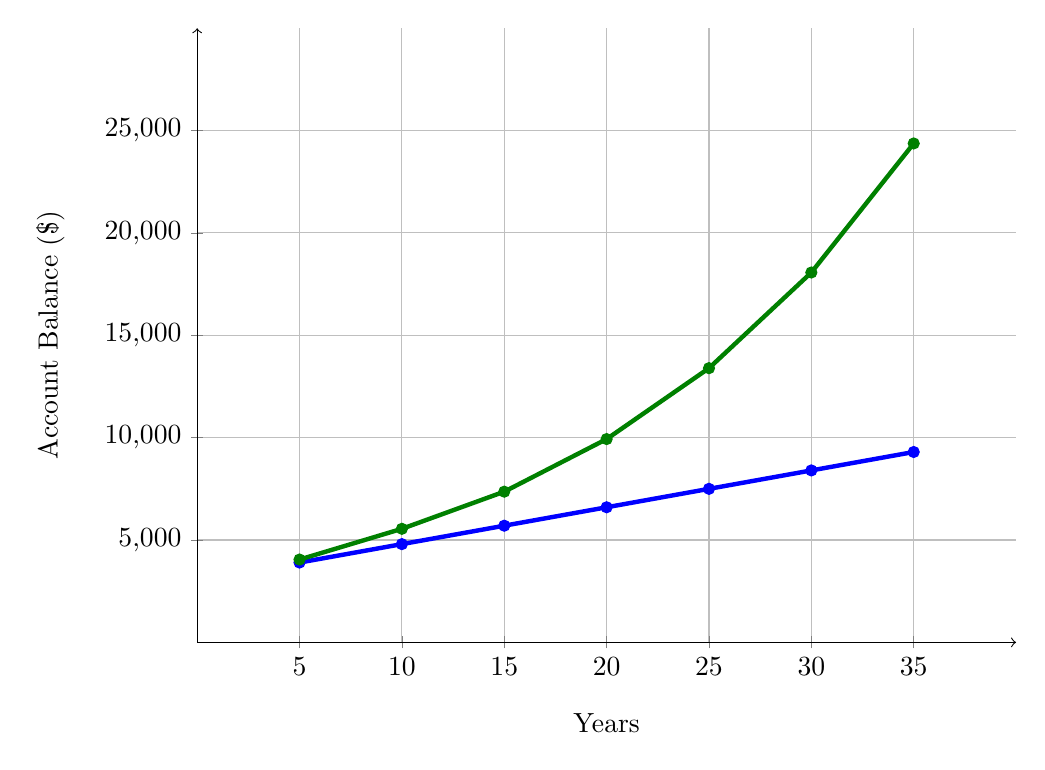
\begin{tikzpicture}
\begin{axis}[
    xmin=0, xmax=40,
    ymin=0, ymax=30,
    axis lines=center,
    axis on top=false,
    domain=0:1,
    x=0.26cm,
    y=0.26cm,
    xtick={5,10,...,35},
    xticklabels={5,10,...,35},
    ytick={0,5,...,25},
    yticklabels={0,{5,000},{10,000},{15,000},{20,000},{25,000},{30,000}},
    axis lines=middle,
    axis line style={->},
    x label style={at={(axis description cs:0.5,-0.1)},anchor=north},
    y label style={at={(axis description cs:-0.15,.5)},rotate=90,anchor=south},
    xlabel={Years},
    ylabel={Account Balance (\$)},
    grid=major
    ]
	\addplot [blue,only marks] table {
	5 3.9
	10 4.8
	15 5.7
	20 6.6
	25 7.5
	30 8.4
	35 9.3
	};
	\addplot [blue,ultra thick] table {
	5 3.9
	10 4.8
	15 5.7
	20 6.6
	25 7.5
	30 8.4
	35 9.3
	};
	\addplot [green!50!black,only marks] table {
	5 4.047
	10 5.548
	15 7.362
	20 9.931
	25 13.395
	30 18.068
	35 24.371
	};
	\addplot [green!50!black,ultra thick] table {
	5 4.047
	10 5.548
	15 7.362
	20 9.931
	25 13.395
	30 18.068
	35 24.371
	};
\end{axis}
\end{tikzpicture}
\end{center}
%\includegraphics[scale=0.65]{SimpleCompoundGraph}
%\end{center}
This illustrates the difference between the linear growth offered by simple interest and the exponential growth offered by compound interest.  Over a long period of time, compounding makes a huge difference.
\end{example}

\begin{proc}{Using Your Calculator: Exponents}
\begin{tabular}{c l}
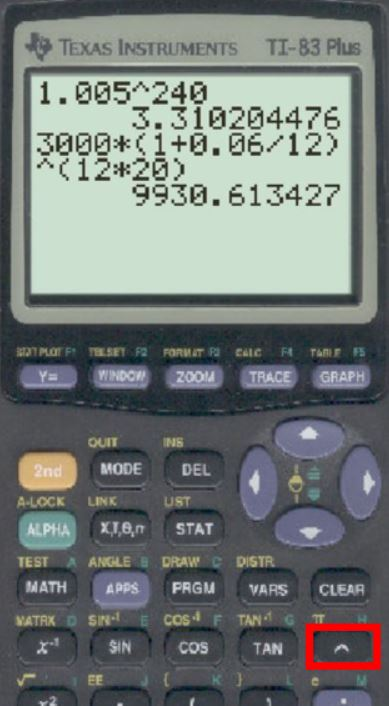
\includegraphics[scale=0.35]{Calculator1} & \parbox[b]{3in}{To evaluate an exponent like $1.005^{240}$ we use the exponent key like the one shown, or possibly $\boxed{y^x}$ or $\boxed{x^y}$ on some calculators.\\  Be careful when evaluating these often-complicated financial formulas; it's usually safer to evaluate them in pieces, like in the first line, where we began by calculating $1+0.06/12 = 1.005$ and $(12)(20)=240$, and then using the exponent key.  If you want to evaluate the entire formula in one step, be careful to use parentheses to do each operation in the proper order, as shown in the second line.\\  Also, be very careful with rounding; keep at least three significant digits (digits after leading zeros) from one calculation to the next, or use the calculator storage function.}
\end{tabular}
\end{proc}

\begin{try}[http://izzomath.com/103text/finance/example3.4/story.html]
If you deposit \$700 at 5\% interest compounded monthly, how much will the account hold in 13 years?
\end{try}
\vfill
\pagebreak

Just like with simple interest, we can use the compound interest formula to answer questions about the present value needed to obtain a given future value.

\begin{example}[https://www.youtube.com/watch?v=pT9iEqWwQ-g]{Saving for College}
You know that you will need \$40,000 for your child's education in 18 years.  If your account earns 4\% compounded quarterly, how much would you need to deposit now to reach your goal?\\

\marginnote{\bfseries Solution}
List the pieces of the formula that are given:
\begin{center}
\begin{tabular}{l l}
$F$ & \$40,000\\
$r$ & 0.04\\
$n$ & 4\\
$t$ & 18
\end{tabular}
\end{center}
In this example, $F$ is given and $P$ is unknown:
\[40,000 = P\left(1+\dfrac{0.04}{4}\right)^{(12)(18)}\]
Solve for $P$:
\[P=\dfrac{40,000}{\left(1+\dfrac{0.04}{4}\right)^{(12)(18)}}=\$19,539.84\]
\end{example}

\begin{try}[http://izzomath.com/103text/finance/example3.5/story.html]
If you want to have \$26,000 in a college fund in 12 years, and you find an account earning 5\% compounded daily, how much should you deposit now?
\end{try}

\begin{proc}{Using Your Calculator: Avoid Rounding If You Can}
In many cases, you can avoid rounding to make your answers more precise based on how you use your calculator.  For example, to calculate something like
\[F = 1000\left(1+\dfrac{0.05}{12}\right)^{(12)(30)}\] start from the inside and work outward.  We can quickly calculate (maybe even mentally) that $(12)(30) = 360$, and now we can use the calculator:
\begin{center}
\begin{tabular}{c | c}
\textbf{Type This} & \textbf{Calculator Shows}\\
\hline
& \\
0.05 $\boxed{\div}$ 12 $\boxed{=}$ & 0.00416666666667\\
& \\
$\boxed{+}$ 1 $\boxed{=}$ & 1.00416666666667\\
& \\
$\boxed{y^x}$ 360 $\boxed{=}$ & 4.46774431400613\\
& \\
$\boxed{\times}$ 1000 $\boxed{=}$ & 4467.74431400613
\end{tabular}
\end{center}
\end{proc}
\pagebreak

\begin{example}[https://www.youtube.com/watch?v=o_iz3lt-GiU]{Don't Round Too Much}
To see why not over-rounding is so important, suppose you were investing \$1000 at 5\% compounded monthly for 30 years.
\begin{center}
\begin{tabular}{l l}
$P$ & \$3000\\
$r$ & 0.06\\
$n$ & 12\\
$t$ & 20
\end{tabular}
\end{center}
To use the formula, we'll need $\frac{r}{n}$, which is 0.0041666666666$\ldots$\\

Notice the effect of rounding this to different values:
\begin{center}
\begin{tabular}{l l l}
$r/n$ rounded: & Gives $F$ to be: & Error\\
\hline
No rounding & \$4467.74 & \\
0.0041667 & \$4467.80 & \$0.06\\
0.004167 & \$4468.28 & \$0.54\\
0.00417 & \$4473.09 & \$5.35\\
0.0042 & \$4521.45 & \$53.71\\
0.004 & \$4208.59 & \$259.15
\end{tabular}
\end{center}
Notice that the error grew by \textit{about} a factor of 10 each time, which is not unusual, considering that we rounded off a digit each time.  

For our purposes, the answer we got by rounding to 0.004167 (four significant digits) is good enough - as long as we're not working in a bank, a rounding error of \$0.54 is fine for us.
\end{example}

\subsection{Comparing Interest Rates}
\begin{example}[https://www.youtube.com/watch?v=8xqmxdrDOcQ]{Comparing Banks}
\marginnote{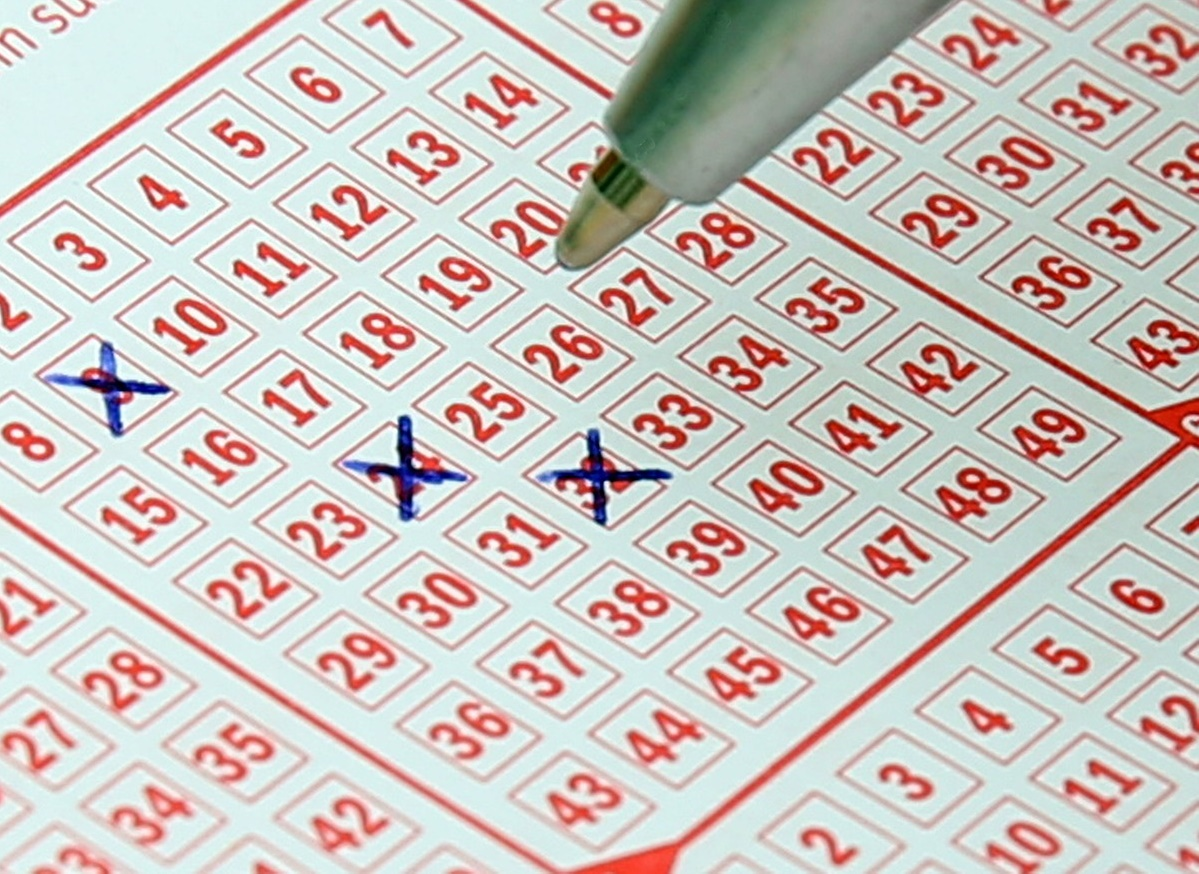
\includegraphics[scale=0.1]{Lottery1}}
You have just won \$500 in the Daily Pick 3 lottery and you decide to deposit your winnings in the bank.  You check with two different banks, which offer different options.  M\&T Bank offers a 4.25\% interest rate compounded daily, while SunTrust offers 4.3\% compounded annually.  Which bank should you choose?\\

\marginnote{\bfseries Solution}
To compare the two banks, simply choose an arbitrary amount of time and calculate how much each account would hold at the end of that time; whichever is higher is the one you'll choose.  Let's pick a year as our length of time, just for simplicity.  The table below shows the results of calculating the future value of your \$500 at the end of a year with each bank.
\begin{center}
\begin{tabular}{c c}
M\&T & SunTrust\\
\hline
& \\
\$521.71 & \$521.50
\end{tabular}
\end{center}
Even though the difference is relatively small, you'll choose the first account, since over time the difference may grow to something more significant.
\end{example}

That example illustrates an important point: you'll often find different loans or accounts expressed in different terms, perhaps with different interest rates and compounding periods.  In that case, you'll want to find some way to put them all on equal footing to compare them; like we did in this example, you can often do a quick calculation to see which will earn more in some arbitrary amount of time.

Banks will often take advantage of the financial illiteracy of their clients to present a loan in terms that will subtly benefit them.  The major goal of this chapter is to turn you into a financially literate and savvy consumer.
\vfill
\pagebreak

\paragraph{Nominal Interest Rate} The \textit{nominal interest rate} is the interest rate that is stated, such as a 3\% annual rate on a bond or a 1.7\% monthly rate on a credit card.

\paragraph{Annual Percentage Rate (APR)} This is the annual nominal rate.  So for instance, the 1.7\% nominal monthly rate would correspond to a $1.7\% \times 12 = 20.4\%$ APR.

\paragraph{Effective Interest Rate} This is the real interest rate.  The \textit{effective rate}, also called the \textit{annual percentage yield (APY)} or the \textit{effective annual yield}, takes the compounding period into account.  This is done by calculating the simple interest rate that would lead to the same growth as that of the compound interest that is offered.\\

In case that's not confusing enough, this doesn't even take into account inflation, or what the rest of the market is doing in general, which are important considerations when investing.

\begin{example}[https://www.youtube.com/watch?v=mkUrRp9le-8]{Calculating the Effective Interest Rate}
You find an account offering 6\% compounded monthly.  What is the effective annual rate?\\

\marginnote{\bfseries Solution}
To find the APY, pick an arbitrary amount of money, and track what the account does for one year.  Let's use \$1000, since it's a nice round sum.  At the end of one year, the account will hold
\[F=\$1000\left(1+\dfrac{0.06}{12}\right)^{(12)(1)} = \$1061.68\]
\paragraph{APY} Now, we need to figure out what interest rate, using simple interest, would make \$1000 grow to \$1061.68 in one year:
\begin{align*}
F &= P(1+rt)\\
1061.68 &= 1000(1+(r)(1))\\
1.06168 &= 1+r\\
0.06168 &= r
\end{align*}
The APY on this account is 6.168\%.
\end{example}

\begin{try}[http://izzomath.com/103text/finance/example3.8/story.html]
If an account offers an APR of 5\% compounded weekly, what is the effective annual interest rate?
\end{try}

\paragraph{APR vs APY} Since APY takes the effect of compounding into account and APR does not, the APY will be slightly higher than the APR for a typical account.  Because of this, banks typically report the APR for debt-related accounts like credit cards and mortgages, and they report the APY for interest-bearing accounts like CDs and money market accounts.\\

Rather than using the procedure in the example above to calculate effective interest rates, we can use a formula to accomplish the same calculation in one step.  It's important to understand, though, that this formula is nothing new; it does exactly what we did in that example, but it does it more quickly.  Thus, if you don't have the formula handy, you can still calculate the effective interest rate as long as you remember that it means the simple interest rate that will lead to the same growth as the compound one after a single year.

\begin{formula}{Effective Annual Yield}
If\marginnote{Using the formula with the numbers from the previous example: \begin{align*}
APY &= \left(1+\dfrac{0.06}{12}\right)^{12}-1\\
&= (1.005)^{12}-1 \\
&= 0.06168
\end{align*}} an account has a nominal annual interest rate of $r$, in decimal form, compounded $n$ times per year, then the effective annual yield, or APY, is given by the following formula.
\[APY = \left(1+\dfrac{r}{n}\right)^n - 1\]
\end{formula}
\vfill
\pagebreak

\begin{example}[https://www.youtube.com/watch?v=P9XX9m4UTdI]{Calculating APY}
A CD offers a nominal interest rate of 4.5\% compounded monthly.  What is the APY for this CD?\\

\marginnote{\bfseries Solution}
Here $r = 0.045$ and $n=12$:
\[APY = \left(1+\dfrac{0.045}{12}\right)^{12} - 1 = 0.04594\]
so the APY is 4.594\%.
\end{example}

\begin{try}[http://izzomath.com/103text/finance/example3.9/story.html]
The APR on a mortgage is 2.83\% compounded monthly.  What is the APY for this mortgage?
\end{try}

\subsection{Continuously Compounded Interest}
We've seen that compound interest makes money grow faster than simple interest does, but we can go even further: if someone offered you an investment compounded monthly and one compounded daily (with everything else equal), which would you choose?  You would be wise to choose the one that is compounded daily, because the more frequently that interest is compounded, the longer that interest that is added has to grow.  In other words, the interest that is added after one day has more time to grow than if it had to wait until the end of the month to be added.

The question is this: is there a limit to this growth?  Could we compound more and more often and see our money grow infinitely?  To answer this, suppose we deposit \$1 for one year into an account with a fixed interest rate---we'll use 100\% to illustrate, even though you'll almost certainly never encounter such an interest rate in real life---and we'll see what happens as we increase $n$, the frequency with which the interest is compounded:
\begin{center}
\begin{tabular}{r r}
$n$ & \hspace{0.5in} $1\left(1+\dfrac{1}{n}\right)^n$\\
\hline
1 & 2.0000000$\ldots$\\
5 & 2.4883200$\ldots$\\
10 & 2.5937424$\ldots$\\
50 & 2.6915880$\ldots$\\
100 & 2.7048138$\ldots$\\
1000 & 2.7169239$\ldots$\\
10,000 & 2.7181459$\ldots$\\
100,000 & 2.7182682$\ldots$\\
1,000,000 & 2.7182804$\ldots$\\
10,000,000 & 2.7182816$\ldots$\\
\end{tabular}
\end{center}

Notice that as we compound more and more frequently, we start to approach a limit.  This limit happens to be a very important number, so important that the letter $e$ is reserved for it.  It forms the basis of exponential growth, which has applications in every field of applied mathematics.\\

For a general interest rate $r$, $\left(1+\dfrac{r}{n}\right)^{nt}$ approaches $e^{rt}$ as the compounding increases.  This is what we call \textit{continously compounded interest}.

\begin{formula}{Continuous Compound Interest}
A present value $P$ will grow to a future value of $F$ under continuous compounding at an interest rate of $r$ according to:
\[F = Pe^{rt}\]
\end{formula}

\begin{proc}{Using Your Calculator: $e$}
\begin{tabular}{c l}
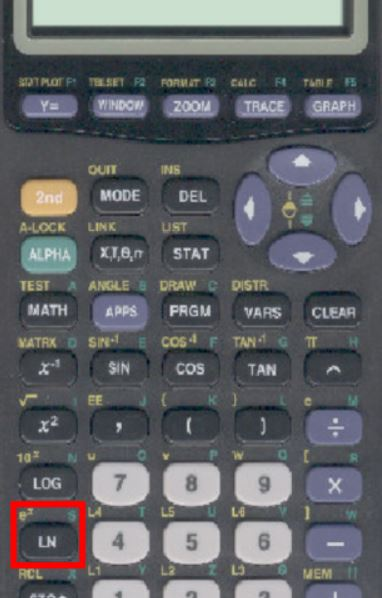
\includegraphics[scale=0.35]{CalculatorE} & \parbox[b]{3in}{Your calculator will most likely have a button for $e$, but depending on what kind of calculator you have, it may look different.\\

Here, the model shown has $e^x$ as the 2nd function of the button marked $\boxed{\textrm{LN}}$\ , so to calculate $e^{0.5}$, for instance, you would press $\boxed{\textrm{2nd}}$\ , then $\boxed{\textrm{LN}}$\ , then enter 0.5, and you should get 1.648721271.\\

On some scientific calculators, you may need to enter 0.5 and then press the $\boxed{e^x}$ key to get the same result.}
\end{tabular}
\end{proc}

\begin{example}[https://www.youtube.com/watch?v=kfZ-xUCgLl8]{Continuous Compound Interest: Future Value}
If you deposit \$4500 in an account paying 3.2\% interest compounded continuously, how much will the account hold after 36 months?\\

\marginnote{\bfseries Solution}
Use the continuous compound formula:
\[F=Pe^{rt} = \$4500e^{(0.032)(3)} = \$4953.42\]
\end{example}

\begin{try}[http://izzomath.com/103text/finance/example3.10/story.html]
If you deposit \$13,000 in an account paying 2.8\% interest compounded continuously, how much will the account hold after 3 years?
\end{try}

Just like we did with other loans, we can also calculate the present value for a given future value.

\begin{example}[https://www.youtube.com/watch?v=vzk6AvZS3h8]{Continuous Compound Interest: Present Value}
How much will you need to deposit today at 5.3\% compounded continuously in order to have \$6300 in 4 years?\\

\marginnote{\bfseries Solution}
Just like before, we'll use the same formula, but now $F$ is known and $P$ is the unknown part.
\begin{align*}
F &= Pe^{rt}\\
\$6300 &= Pe^{(0.053)(4)}\\
\$6300 &= P(1.2361)\\
\dfrac{\$6300}{1.2361} &= P\\
\$5096.48 &= P
\end{align*}
\end{example}

\begin{try}[http://izzomath.com/103text/finance/example3.11/story.html]
How much will you need to deposit today at 3.6\% compounded continuously in order to have \$1200 in 5 years?
\end{try}
\vfill
\pagebreak

\begin{example}[https://www.youtube.com/watch?v=OuC95ArdH5g]{Comparing Different Compounding Periods}
You have \$7000 to invest for 5 years.  Find how much you'll have at the end of the 5 years if you earn 4\% compounded
\begin{enumerate}[(a)]
\item annually
\item monthly
\item daily
\item continuously
\end{enumerate}
\vspace{0.2in}

\marginnote{\bfseries Solution}
The first three all use the same formula, and all that changes is $n$:
\begin{enumerate}[(a)]
\item Compounded annually:
\begin{align*}
F &= P\left(1+\dfrac{r}{n}\right)^{nt}\\
&= 7000\left(1+\dfrac{0.04}{1}\right)^{(1)(5)}\\
&= \$8516.57
\end{align*}

\item Compounded monthly:
\begin{align*}
F &= P\left(1+\dfrac{r}{n}\right)^{nt}\\
&= 7000\left(1+\dfrac{0.04}{12}\right)^{(12)(5)}\\
&= \$8546.98
\end{align*}

\item Compounded daily:
\begin{align*}
F &= P\left(1+\dfrac{r}{n}\right)^{nt}\\
&= 7000\left(1+\dfrac{0.04}{365}\right)^{(365)(5)}\\
&= \$8549.73
\end{align*}

\item Compounded continuously:
\begin{align*}
F &= Pe^{rt}\\
&= 7000e^{(0.04)(5)}\\
&= \$8549.82
\end{align*}
\end{enumerate}
\end{example}

\begin{try}[http://izzomath.com/103text/finance/example3.12/story.html]
If you deposit \$300, how much will you have in 7 years if you receive 3.5\% interest compounded
\begin{enumerate}[(a)]
\item quarterly?
\item monthly?
\item weekly?
\item continuously?
\end{enumerate}
\end{try}
\vfill
\pagebreak

\paragraph{Doubling Time} One common measure used to quickly compare investments is to determine how long it will take to double an investment.  The shorter the doubling time, the better the investment.

\begin{proc}{Solving Exponential Equations}
To solve an exponential equation, we use logarithms.  For exponential equations, we'll use the \textit{natural logarithm}, $\ln$.
\[\textrm{If } e^x = y, \textrm{ then } x = \ln y\]
\end{proc}

We can use this to solve equations where we know the present value, and we want to find the amount of time to reach a given future value.  Once we get to \[\dfrac{F}{P}=e^{rt}\] we'll use the natural logarithm to extract the exponent $rt$:
\[\ln \dfrac{F}{P} = rt\]

Since we can evaluate the expression on the left with a calculator, we can get an answer for $t$, the amount of time it will take for $P$ dollars to grow to $F$ dollars.

\begin{example}[https://www.youtube.com/watch?v=WKByWayHv00]{Doubling Time}
Find the time required to double an investment at 6\% interest compounded continuously.\\

\marginnote{\bfseries Solution}
We could again pick an arbitrary amount for $P$, and let $F$ be double that.  Instead, though, we'll simply replace $F$ with $2P$, and solve the formula for $t$:
\begin{align*}
F &= Pe^{rt}\\
2P &= Pe^{0.06t}\\
2 &= e^{0.06t}\\
\ln 2 &= 0.06t\\
\dfrac{\ln 2}{0.06} &= t\\
11.55 &= t
\end{align*}
Thus the investment will take approximately 11.5 years to double.
\end{example}

\begin{try}[http://izzomath.com/103text/finance/example3.13/story.html]
How long will it take an investment to double at 5\% compounded continuously?
\end{try}

\begin{proc}{Doubling Time}
A quick back-of-the-envelope way to approximate doubling time is to divide 72 by the percent interest rate (i.e. not the decimal form, but 100 times that).  So for example, with an interest rate of 6\%:
\[\textrm{Doubling Time } \approx \dfrac{72}{6} = 12\]
\end{proc}
\pagebreak

\subsection{Inflation}
During inflation, prices increase.  While this growth is usually not constant, if we approximate short periods of inflation as increasing at a constant rate, we can use the compound interest formula to model it.

\begin{example}[https://www.youtube.com/watch?v=gNp9Dlq-ksk]{Inflation}
Suppose that there is constant 4\% inflation from mid-2015 through mid-2020.  What will the projected price be in mid-2020 for an item that costs \$150 in mid-2015?\\

\marginnote{\bfseries Solution}
Use the compound interest formula with $P=\$150$, $r=0.04$, $n=1$, and $t=5$:
\[F=\$150\left(1+\dfrac{0.04}{1}\right)^{(1)(5)} = \$182.50\]
\end{example}

\begin{try}[http://izzomath.com/103text/finance/example3.14/story.html]
If there is constant 3\% inflation from 2015 to 2018, what will a \$85 item in 2015 cost in 2018?
\end{try}

Inflation can also be thought of as a depreciating dollar; in other words, a dollar will buy less next year than it buys now.  It turns out we can still use the compound interest formula, but now the ``interest rate''---actually the rate of depreciation---is negative.

Suppose, for illustration, that inflation is 25\%.  What costs \$100 today will cost \$125 in a year, so a dollar will only buy 80\% of what a dollar can buy today (\$100/\$125).  Thus, the depreciation rate is 20\%.  In general, if $i$ is the rate of inflation, the rate of depreciation (taken as negative) is
\[d=\dfrac{i}{1+i}.\]

Therefore, to calculate the future value of a dollar under inflation, we can use the compound interest formula with $n=1$ and $r=-\dfrac{i}{1+i}$:
\[F=P\left(1-\dfrac{i}{1+i}\right)^t\]

\begin{example}[https://www.youtube.com/watch?v=bNXuphP1Yc4]{Depreciating Dollars}
If there is constant 4\% inflation from mid-2015 through mid-2020, what will the value of a 2020 dollar be in terms of 2015 dollars?\\

\marginnote{\bfseries Solution}
Since inflation is occurring at 4\%, \[d=\dfrac{0.04}{1.04} = 0.03846,\] so using the compound interest formula: 
\[F=\$1(1-0.03846)^5 = \$0.82\]  Thus, a dollar in 2015 will only be worth \$0.82 five years later.
\end{example}

\begin{try}[http://izzomath.com/103text/finance/example3.15/story.html]
If there is constant 3\% inflation from 2015 to 2018, what will the value be of a 2018 dollar in terms of 2015 dollars?
\end{try}

In reality, inflation does not actually occur at a constant rate.  Thus, rather than using the compound interest formula to evaluate inflation, the US Bureau of Labor Statistics measures the cost of common goods periodically and compares the results to costs at other points in time to determine how inflation has changed the value of a dollar.  It is not a perfect system by any means, but it can give a good approximation for the value of a dollar in comparison to other years.

This process creates the Consumer Price Index (CPI), and each month the CPI is recorded; we'll use the average annual CPI for our examples.  Recently, the base years are taken as 1982-1984, so the average index for 1982-1984 is set to 100.  The table below records the CPI for each year from 1980 to 2003.
\begin{center}
\label{CPI Table}
\begin{tabular}{c r | c r | c r}
\textbf{Year} & CPI & \textbf{Year} & CPI & \textbf{Year} & CPI\\
\hline
& & & & & \\
\textbf{1950} & 24.1 & \textbf{1968} & 34.8 & \textbf{1986} & 109.6\\
\textbf{1951} & 26.0 & \textbf{1969} & 36.7 & \textbf{1987} & 113.6\\
\textbf{1952} & 26.6 & \textbf{1970} & 38.8 & \textbf{1988} & 118.3\\
\textbf{1953} & 26.7 & \textbf{1971} & 40.5 & \textbf{1989} & 124.0\\
\textbf{1954} & 26.9 & \textbf{1972} & 41.8 & \textbf{1990} & 130.7\\
\textbf{1955} & 26.8 & \textbf{1973} & 44.4 & \textbf{1991} & 136.2\\
\textbf{1956} & 27.2 & \textbf{1974} & 49.3 & \textbf{1992} & 140.2\\
\textbf{1957} & 28.1 & \textbf{1975} & 53.8 & \textbf{1993} & 144.5\\
\textbf{1958} & 28.9 & \textbf{1976} & 56.9 & \textbf{1994} & 148.2\\
\textbf{1959} & 29.1 & \textbf{1977} & 60.6 & \textbf{1995} & 152.4\\
\textbf{1960} & 29.6 & \textbf{1978} & 65.2 & \textbf{1996} & 156.9\\
\textbf{1961} & 29.9 & \textbf{1979} & 72.6 & \textbf{1997} & 160.5\\
\textbf{1962} & 30.9 & \textbf{1980} & 82.4 & \textbf{1998} & 163.0\\
\textbf{1963} & 30.6 & \textbf{1981} & 90.9 & \textbf{1999} & 166.6\\
\textbf{1964} & 31.0 & \textbf{1982} & 96.5 & \textbf{2000} & 172.2\\
\textbf{1965} & 31.5 & \textbf{1983} & 99.6 & \textbf{2001} & 177.1\\
\textbf{1966} & 32.4 & \textbf{1984} & 103.9 & \textbf{2002} & 179.9\\
\textbf{1967} & 33.4 & \textbf{1985} & 107.6 & \textbf{2003} & 184.0\\
\end{tabular}
\end{center}

To compare costs from two different years, use the ratio of the CPI in those two years:
\[\dfrac{\textrm{Cost in Year A}}{\textrm{Cost in Year B}} = \dfrac{\textrm{CPI for Year A}}{\textrm{CPI for Year B}}\]

\begin{example}[https://www.youtube.com/watch?v=tJS3kwwr8XA]{Using the CPI}
If a home cost \$190,000 in 1986, approximately what would the same home cost in 2002?\\

\marginnote{\bfseries Solution}
\marginnote{
\includegraphics[scale=0.08]{House1}}
Use the proportion given above, along with the CPI table:
\begin{align*}
\dfrac{\textrm{Cost in 2002}}{\textrm{Cost in 1986}} &= \dfrac{\textrm{CPI for 2002}}{\textrm{CPI for 1986}}\\
&\\
\dfrac{\textrm{Cost in 2002}}{\$190,000} &= \dfrac{179.9}{109.6}
\end{align*}
Then, \[\textrm{Cost in 2002} = \$190,000 \times \dfrac{179.9}{109.6} \approx \$311,870\marginnote{Note: $\approx$: ``approximately''}\]
\end{example}

\begin{try}[http://izzomath.com/103text/finance/example3.16/story.html]
If a home cost \$235,000 in 1998, use the CPI table to determine how much the same home would have cost in 1978.
\end{try}

\begin{exercises}
\textit{In Exercises 1---4, a principal amount is borrowed at the given interest rate for the given period of time.  Find the loan's future value $F$, or the amount due at the end of the time, if the loan uses simple interest.}

\pfour{\begin{tabular}{r l}
Principal: & \$3000\\
Interest rate: & 7\%\\
Time: & 2 years
\end{tabular}}
\pfour{\begin{tabular}{r l}
Principal: & \$2700\\
Interest rate: & 4\%\\
Time: & 3 years
\end{tabular}}
\pfour{\begin{tabular}{r l}
Principal: & \$7500\\
Interest rate: & 3.5\%\\
Time: & 18 months
\end{tabular}}
\pfour{\begin{tabular}{r l}
Principal: & \$1600\\
Interest rate: & 4.85\%\\
Time: & 36 months
\end{tabular}}

\textit{In Exercises 5---8, a principal amount is borrowed at the given interest rate for the given period of time.  If the future value is given, find the principal if the loan uses simple interest.}

\pfour{\begin{tabular}{r l}
Future value: & \$9000\\
Interest rate: & 5.5\%\\
Time: & 1 year
\end{tabular}}
\pfour{\begin{tabular}{r l}
Future value: & \$7700\\
Interest rate: & 6\%\\
Time: & 4 years
\end{tabular}}
\pfour{\begin{tabular}{r l}
Future value: & \$800\\
Interest rate: & 2.75\%\\
Time: & 9 months
\end{tabular}}
\pfour{\begin{tabular}{r l}
Future value: & \$1450\\
Interest rate: & 5.3\%\\
Time: & 24 months
\end{tabular}}

\textit{In Exercises 9---11, a principal amount is borrowed at the given interest rate for the given period of time, and interest is compounded as stated.  Find the loan's future value $F$, or the amount due at the end of the time.}

\pthree{\begin{center}\begin{tabular}{r l}
Principal: & \$1200\\
Interest rate: & 5\%\\
Compounding: & Annually\\
Time: & 3 years
\end{tabular}\end{center}}
\pthree{\begin{tabular}{r l}
Principal: & \$5700\\
Interest rate: & 3.5\%\\
Compounding: & Monthly\\
Time: & 24 months
\end{tabular}}
\pthree{\begin{tabular}{r l}
Principal: & \$3000\\
Interest rate: & 5.32\%\\
Compounding: & Continuously\\
Time: & 48 months
\end{tabular}}

\textit{In Exercises 12---14, a principal amount is borrowed at the given interest rate for the given period of time, and interest is compounded as stated.  If the future value is given, find the principal.}

\pthree{\begin{tabular}{r l}
Future value: & \$17,500\\
Interest rate: & 3\%\\
Compounding: & Annually\\
Time: & 8 years
\end{tabular}}
\pthree{\begin{tabular}{r l}
Future value: & \$18,000\\
Interest rate: & 5.6\%\\
Compounding: & Daily\\
Time: & 18 months
\end{tabular}}
\pthree{\begin{tabular}{r l}
Future value: & \$9000\\
Interest rate: & 7.48\%\\
Compounding: & Continuously\\
Time: & 60 months
\end{tabular}}

\ptwo{A friend lends you \$200 for a week, which you agree to repay with 5\% one-time interest. How much will you have to repay?}
\ptwo{Suppose you obtain a \$3,000 T-note with a 3\% annual rate, paid quarterly, with maturity in 5 years.  How much interest will you earn?}

\ptwo{A student took out a simple interest loan for \$2,400 for two years at an annual rate of 7\%.  
\begin{enumerate}[(a)]
\item What is the interest on the loan?
\item How much will the student have to repay at the end of two years?
\end{enumerate}
}
\ptwo{A loan of \$2,040 has been made at a 5.7\% annual simple interest rate for four months.  
\begin{enumerate}[(a)]
\item What is the interest on the loan?
\item Find the future value of the loan.
\end{enumerate}}

\ptwo{You deposit \$2000 in an account earning 3\% interest compounded monthly.
\begin{enumerate}[(a)]
\item How much will you have in the account in 20 years?
\item How much interest will you earn?
\end{enumerate}}
\ptwo{You deposit \$10,000 in an account earning 4\% interest compounded weekly.
\begin{enumerate}[(a)]
\item How much will you have in the account in 25 years?
\item How much interest will you earn?
\end{enumerate}}

\ptwo{How much would you need to deposit in an account earning 6\% compounded monthly in order to have \$6,000 in the account in 8 years?}
\ptwo{How much would you need to deposit in an account earning 5\% compounded quarterly in order to have \$20,000 in the account in 4 years?}

\ptwo{If you deposit \$5400 in an account earning 4.35\% interest compounded continuously, how much will the account hold in 18 months?}
\ptwo{If you take out a loan for \$7700 at 6.7\% interest compounded continously, how much will you have to pay back in 5 years?}

\ptwo{How much do you need to deposit today at 4\% interest compounded continuously in order to have \$4000 in 2 years?}
\ptwo{If you find a CD offering 5.8\% interest compounded continuously, how much should you deposit if you are saving up to refinish your kitchen in 3 years and you estimate that will take \$15,000?}

\ptwo{If a mortgage is advertised with a 3.12\% APR, compounded monthly, what is the APY on this mortgage?  Which is the bank more likely to present to their clients?}
\ptwo{If the APR on a retirement account is 4.4\%, compounded quarterly, what is the APY?  Which is the bank more likely to advertise?}

\ptwo{You have \$12,000 to invest for 3 years.  Find how much you'll have at the end of the 3 years if you earn 4\% interest compounded
\begin{enumerate}[(a)]
\item annually
\item monthly
\item daily
\item continuously
\end{enumerate}}
\ptwo{You would like to have \$8000 saved in 3 years.  Find how much you'll have to invest now to reach that goal if you earn 6\% interest compounded
\begin{enumerate}[(a)]
\item annually
\item monthly
\item daily
\item continuously
\end{enumerate}}

\ptwo{How long will it take to double an investment at 7\% compounded annually?}
\ptwo{How long will it take to double an investment at 4.6\% compounded continuously?}

\ptwo{Suppose that there is constant 3.5\% inflation from 2015 to 2025.  What is the projected 2025 price for an item that costs \$357 in 2015?}
\ptwo{If there is constant 3.5\% inflation from 2015 to 2025, what will the value of a 2025 dollar be in terms of 2015 dollars?}

\ptwo{Use the CPI table on page \pageref{CPI Table} to estimate the cost of a gallon of milk in 1998 if it cost \$2.22 in 1986.  What percentage increase is this?}
\ptwo{Use the CPI table on page \pageref{CPI Table} to estimate the average cost of a dozen eggs in 1986 if it cost \$1.09 in 1998.  What percentage increase is this?}

\end{exercises}
